\documentclass[tikz,border=5]{article}
\usepackage[utf8]{inputenc}
\usepackage{amsfonts}
\usepackage{amsmath}
\usepackage{amssymb}
\usepackage{amsthm}
\usepackage{indentfirst}
\usepackage{multicol}
\usepackage{xcolor}
\usepackage{tikz}
\usetikzlibrary{trees}
\theoremstyle{definition}
\newtheorem{exerc}{Questão}

\title{Prova 1 Lógica para Computação - MATA47}
\author{João Lucas Lima de Melo}

\begin{document}
	\maketitle
	\begin{exerc} Seja a fórmula $\varphi = x \vee \neg y \rightarrow x \rightarrow z$. As subfórmulas e as inserções de parênteses de $\varphi$ são dadas por:
	    \begin{displaymath}
	        x \vee \neg y \rightarrow x \rightarrow z
	    \end{displaymath}
	    \begin{displaymath}
	        (x \vee \neg y) \rightarrow x \rightarrow z
	    \end{displaymath}
	    \begin{displaymath}
	        (x \vee \neg y) \rightarrow (x \rightarrow z)
	    \end{displaymath}
	    \begin{displaymath}
	        \varphi = ((x \vee \neg y) \rightarrow (x \rightarrow z))
	    \end{displaymath}
	    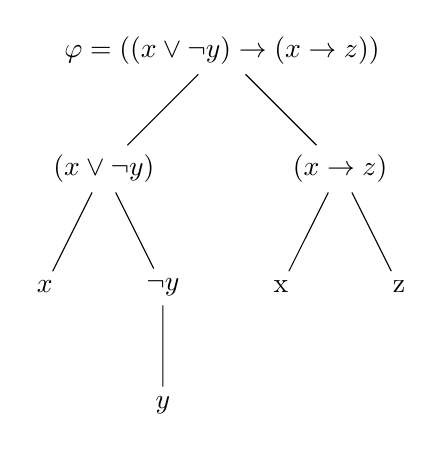
\begin{tikzpicture}[
			level distance=1.5cm,
			level 1/.style={sibling distance=3cm},
			level 2/.style={sibling distance=1.5cm}]
			\node {$\varphi = ((x \vee \neg y) \rightarrow (x \rightarrow z))$}
			child {node {$(x \vee \neg y)$}
			    child {node {$x$}}
			    child {node{$\neg y$}
			        child {node{$y$}}
			    }
			}
			child {node {$(x \rightarrow z)$}
				child {node{x}}
				child {node{z}}
			};	
		\end{tikzpicture}
		
	\end{exerc}
	\begin{exerc}[Fórmulas do Exemplo 3.5 do script.]
		Seja $\varphi = (\psi \wedge \chi)$. Pela hipótese da indução, $\psi$ tem um número par de parênteses que vamos chamar de 2m. Também pela hipótese, temos que $\chi$ tem um número par de parênteses que chamaremos de 2n. Logo $\varphi$ tem um número de parênteses igual à $2 + 2n + 2m = 2(1+n+m)$. Este número é par.
		
		Seja $\varphi = (\psi \rightarrow \chi)$. Pela hipótese da indução, $\psi$ tem um número par de parênteses que vamos chamar de 2m. Também pela hipótese, temos que $\chi$ tem um número par de parênteses que chamaremos de 2n. Logo $\varphi$ tem um número de parênteses igual à $2 + 2n + 2m = 2(1+n+m)$. Este número é par.
	\end{exerc}
	\begin{exerc}[Exercício 3.8(a)]
		Seja M um conjunto, $S \subseteq M$ um subconjunto de M, $Pw(M)$ o conjunto potência de M, e $\chi$ um elemento de $Pw(M)$. $\left \{ 0,1 \right \}^M$ é o conjunto dado por funções que podem ser descritas por $f_s:M \rightarrow  \left \{ 0,1 \right \}, f_s:= m \mapsto \begin{Bmatrix}
			1, m\in  S,\, S \subseteq M \\0, c.c. \end{Bmatrix}$(chamada de funções indicativas ou características). Podemos criar a função que relaciona $f_s$  e $\chi$:$\newline h:\left \{ 0,1 \right \}^M \rightarrow Pw(M)
		\newline h:= f_s \mapsto \chi, se \: s = \chi.$ Essa função é bijetora pelo fato de que, para cada s em $\left \{ 0,1 \right \}^M$, existe um $\chi$ igual em $Pw(M)$. 
	\end{exerc}
	\begin{exerc}
	    $ $
	    \begin{enumerate}
	    	\item i $\Rightarrow$ ii \newline Seja $\Phi$ insatisfazível, ou seja, $Mod(\Phi) = \varnothing$ \newline Por definição de consequência lógica,
	    	\begin{center} $\Phi \Vdash \varphi$ se $Mod(\Phi) \subseteq Mod(\{\varphi\})$ \end{center} Por definição, $\varnothing$ está contido em qualquer conjunto. \newline Portanto, $\forall \varphi$, $Mod(\Phi) \subseteq Mod(\{\varphi\})$, ou seja: \begin{center} $\Phi \Vdash \varphi, \forall \varphi \in \Phi$  \end{center}

	        \item ii $\Rightarrow$ iii \newline Seja $\Phi$ um conjunto de fórmulas e uma fórmula $\varphi$ tal que \begin{center}$\Phi \Vdash \varphi, \forall \varphi \in \Phi$ \end{center} Assumindo $\varphi = \perp$, podemos afirmar, pela hipótese adotada que \begin{center} $\Phi \Vdash \perp$ \end{center} 
	        
	        \item iii $\Rightarrow$ i \newline Seja $\Phi$ um conjunto de fórmulas tal que \begin{center} $\Phi \Vdash \perp$ \end{center} Por definição de consequência lógica, \begin{center} $\Phi \Vdash \perp$ se $Mod(\Phi) \subseteq Mod(\{\perp\})$ \end{center} Por definição de modelo, temos \begin{center} $Mod(\Phi) := \{v \in 2^{v} |v \vDash \Phi\}$ \end{center} No entando, no caso de $\{\perp\}$, $\perp$ nunca é satisfeita por nenhuma valoração. Ou seja, \begin{center} $v \nvDash \perp :\Leftrightarrow v(\perp) = 0$, logo\end{center}\begin{center} $Mod(\{\perp\}) = \varnothing$ \end{center} Como \begin{center} $\Phi\ \Vdash\perp$ e \end{center} \begin{center}$\phi\Vdash\perp$ se $Mod(\Phi) \subseteq Mod(\{\perp\})$ e \end{center}\begin{center} $Mod(\{\perp\}) = \varnothing$ \end{center} Temos que \begin{center} $Mod(\Phi) = \varnothing$ \end{center}
	    \end{enumerate}
	\end{exerc}
	\begin{exerc}
	    $ $
	    \begin{enumerate}
	        \item $\Vdash \varphi$ \newline Para toda $v \in 2^{V}, v \vDash \varnothing$ (uma vez que para $v \vDash \Phi$, para um conjunto de fórmulas $\Phi$, é necessário que $v \vDash \varphi, \forall \varphi \in \Phi$. Como $\nexists \varphi \in \varnothing, v \vDash \varnothing$). \newline Portanto, basta que $Mod(\{\varphi\})$($\varphi$ seja válida) para que $\Vdash \varphi$
	        \item $\{\varphi\} \Vdash \varphi \vee \psi$ \newline Seja $v \in 2^{v}$ tal que $v \vDash \varphi$. De imediato, pela definição de $\vee$, segue que $v \vDash \varphi \vee \psi$
	        \item $\{\varphi, \varphi \rightarrow \psi\} \Vdash \psi$ \newline Seja $v \in 2^{V}$ tal que $v \vDash \varphi$ e $v \vDash \varphi \rightarrow \psi$ \newline A partir de $v \vDash \varphi \rightarrow \psi$, pela definição de $\rightarrow$, temos \begin{center} $v \nvDash \varphi$ ou \end{center} \begin{center} $v \vDash \psi$ \end{center} Como, por hipótese, $v \vDash \varphi$, então: \begin{center} $v \vDash \psi$ \end{center}
	        \item $\{\varphi \rightarrow \psi\} \Vdash (\chi \vee \varphi) \rightarrow (\chi \vee \psi)$ \newline Seja $v \in 2^{V}$ tal que $v \vDash \varphi \rightarrow \psi$ \newline A partir de $v \vDash \varphi \rightarrow \psi$, pela definição de $\rightarrow$, temos: \begin{enumerate}
	            \item $v \nvDash \varphi$ \newline Se $v \vDash \chi$, então $v \vDash (\chi \vee \varphi)$ e $v \vDash (\chi \vee \psi)$. Assim, vale a consequência lógica. \newline Se $v \nvDash \chi$, então $v \nvDash (\chi \vee \varphi)$. Pela definição de $\rightarrow$, portanto, $v \vDash (\chi \vee \varphi) \rightarrow (\chi \vee \psi)$ e, portanto, valeria a consequência lógica.
	            \item $v \vDash \psi$ \newline Então, $v \vDash \chi \vee \psi$. Portanto, valeria a sequência lógica.
	        \end{enumerate}
	        Vale a sequência lógica.
	        \item $\{(\varphi \wedge \psi) \rightarrow \chi, \theta \rightarrow \psi\} \Vdash (\varphi \wedge \theta) \rightarrow \chi$ \newline Seja $v \in 2^{V}$ tal que $v \vDash (\varphi \wedge \psi) \rightarrow \chi$ e $v \vDash \theta \rightarrow \psi$ \newline A partir de $v \vDash (\varphi \wedge \psi) \rightarrow \chi$ e pela definição de $\rightarrow$ e $\wedge$, temos:
	        \begin{enumerate}
	            \item $v \vDash \psi$ \newline Nesse caso, pela definição de $\wedge$, temos: \begin{center} $v \nvDash (\varphi \wedge \psi) \rightarrow \chi$ \end{center} Já que não satisfaz o consequente, satisfazendo o antecedente.
	            \item $v \vDash \psi$ \newline Nesse caso, pela definição de $\rightarrow$, temos: \begin{center} $v \nvDash \theta \rightarrow \psi$ \end{center} Já que não satisfaz o antecedente, satisfazendo o consequente.
	        \end{enumerate}
	        Portanto, podemos afirmar que \begin{center} $\exists \alpha \in \{(\varphi \wedge \psi) \rightarrow \chi, \theta \rightarrow \psi\}$ tal que $v \nvDash \alpha$ \end{center} Logo, não vale a sequência lógica.
	    \end{enumerate}
	\end{exerc}
	\begin{exerc}
		Sejam $\varphi, \psi, \chi \in F_m$ tal que $\varphi = \psi \wedge \chi.$ Supomos que $v_1(\psi)$ = $v_2(\psi)$ e $v_1(\chi)$ = $v_2(\chi)$ (por hipótese). Aplicando a definição de $v_1(\varphi) = v_1(\psi \wedge \chi)$ (por def.) $= f_{\wedge}(v_1(\psi), v_1(\chi))$, usando a hipótese $f_{\wedge}(v_1(\psi), v_1(\chi)) = f_{\wedge}(v_2(\psi), v_2(\chi))$, que por definição, é $v_2(\psi \wedge \chi)$ que é $v_2(\varphi)$. o que prova a indução.
		\newline Sejam $\varphi, \psi, \chi \in F_m$ tal que $\varphi = \psi \vee \chi.$  Supomos que $v_1(\psi)$ = $v_2(\psi)$ e $v_1(\chi)$ = $v_2(\chi)$ (por hipótese). Aplicando a definição de $v_1(\varphi) = v_1(\psi \vee \chi)$ (por def.) $= f_{\vee}(v_1(\psi), v_1(\chi))$, usando a hipótese $f_{\vee}(v_1(\psi), v_1(\chi)) = f_{\vee}(v_2(\psi), v_2(\chi))$, que por definição, é $v_2(\psi \vee \chi)$ que é $v_2(\varphi)$. o que prova a indução.
		\newline Sejam $\varphi, \psi, \chi \in F_m$ tal que $\varphi = \psi \rightarrow \chi.$  Supomos que $v_1(\psi)$ = $v_2(\psi)$ e $v_1(\chi)$ = $v_2(\chi)$ (por hipótese). Aplicando a definição de $v_1(\varphi) = v_1(\psi \rightarrow \chi)$ (por def.) $= f_{\rightarrow}(v_1(\psi), v_1(\chi))$, usando a hipótese $f_{\rightarrow}(v_1(\psi), v_1(\chi)) = f_{\rightarrow}(v_2(\psi), v_2(\chi))$, que por definição, é $v_2(\psi \rightarrow \chi)$ que é $v_2(\varphi)$. o que prova a indução.		
	\end{exerc}
\end{document}
